\section{Changing of workflows} \label{changeofworkflows}

With the evolution form Centralized Version Control System to Distributed Version Control Systems there also 
evolved new ways of how development processes can be organized. In this section we want to show differences 
between centralized and distributed systems, especially we work with them, where problem can occur by using 
centralized systems and how the distributed systems try to solve them. At the the end of the section we want 
to show some common models to handle projects of different sizes.

\subsection{Workflow differences}

The difference which has the most impact on how we work with the systems is the centralized/distributed aspect. 
A distributed system saves the whole project history locally, also all operations are performed on the local clone. 
This is a huge advantage over centralized systems. A developer does not have to be connected to the central 
repository to work on a project. Maybe thats not 100 percent true. The developer can work on his project, but 
he can not work with the version control system. So the distributed systems have a “mobile” advantage. 
Developers can work on their projects wherever they are and there is no need for a connection with the 
Internet or the company network.

It is not only about the remote connection, it is also about the server availability. If the server, where 
all the repositories are hosted, goes offline for whatever reason, all developers are cut off from development.

Because centralized systems have to talk with their servers for many operations they work not as fast as 
a distributed system does. It does take a lot more time to checkout a previous version over the network 
then reverting back to a previous version locally. This fact has an impact on how developers use the system. 
If operations are very fast and take only little time developers may use them more often. They may commit 
more often not only because its fast, but because their commit can not break the whole project. 
In centralized environments every developer “must” commit only code which is stable so the project 
itself stays in a stable state. The implication of this need for stable commits is that developers won't 
commit for a longer time so their code base diverges more from the main line and it is very hard 
to merge the changes back to the main line.

The next big difference is the aspect of branching and merging. It is not so common to use branches 
in centralized systems then it is in distributed ones. SVN for example doest not have a separate branch 
mechanism at all.
It is the task of the SVN administrator to organize the main line, branches and tags on the server. 
So it is very hard to create a branch just to implement some new feature or to fix a single bug. Another 
point is that all the branches are visible and accessible for everyone. So there can only 
be one branch called “test”.

As the reader may see in the section about git, it is very common in distributed environments to 
do a lot of branching and merging. The reason for this is that DVCS like Mercurial, Git and Baazar 
have the design goal to make branching and merging easy and fast. So a developer may create a branch 
for each issue in the issue tracker. When he has solved the issue he merge the fix back to the main 
line and delete the branch. Thats also true for new or experimental features or just for some sort 
of testing purpose. Nobody will ever know that there was a branch except the developer publishes 
it and allows other developers to pull his branch into their local repository. If they do so, it 
does not mean that they have to merge the branches or use the branch at all. If someone delete 
the branch locally, nobody cares.


\subsection{Distributed workflow models}

These models were described in the Pro Git Book \footnote{http://progit.org/book/ch5-1.html} and are 
worth mentioned here. The images are also adopted from the book but made a little bit smaller and more compact.

In a distirbuted environment every developer acts as a contributor and as a server at the same time. So there are more 
possibilities to organize development processes then there are are in a centralized environment.


\subsubsection{Centralized Model}

\begin{figure}[ht]
  \centering
  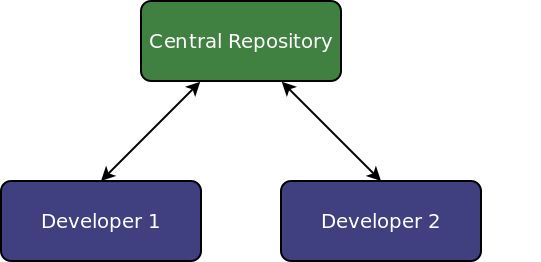
\includegraphics[width=0.5\textwidth]{img/Mod_Central}
  \caption{Centralized Model}
  \label{fig:mod_centralized} 
\end{figure}

First of all you can use a DCVS like a normal centralized system (see Figure \ref{fig:mod_centralized}). One developers repository or a extra repository acts as the central hub. Before a developer can push his work to the central repository he has to merge all the changes done to the central repository into his local repository. This model works well for small project teams as well as for people who come from a centralized background and are not familiar with distributed workflows.


\subsubsection{Integration-Manager Workflow}

\begin{figure*}[tbp]
  \centering
  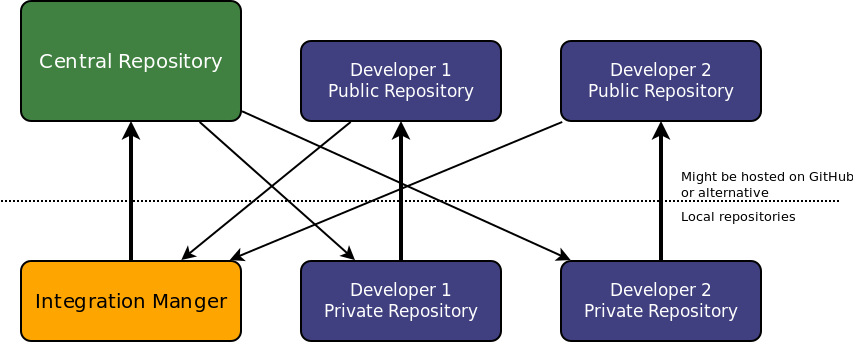
\includegraphics[width=\textwidth]{img/Mod_IntegrationManager}
  \caption{Model with an Integration Manager}
  \label{fig:mod_intMan} 
\end{figure*}

This workflow becomed very common as sites like GitHub started to evolve. In
this model (see Figure \ref{fig:mod_intMan}) just a handful of people has write access to the central (or “official”) repository. 
This people are called integration managers. In smaller projects there might be just one integration manager and their 
number may grow with the project size. The task of an integration manager is to pull changes from developers and merge 
them into the central repository. They also have to decide which changes are worth merging.

Every developer has also a public repository, so the integration managers and the other developers can easily pull from 
each other. The real work is done in the private local repositories from the developers. Once changes are merged into the 
official repository the developers have to merge them back into their private repositories, so they have the same state as the official one.

This model works very well in open source projects, because its possible to host OSS (Open Source Software) on 
sites like GitHub for free, so the public repositories from the developers and the integration managers might be hosted there.


\subsubsection{Dictator and Lieutenants Workflow}

\begin{figure}[ht]
  \centering
  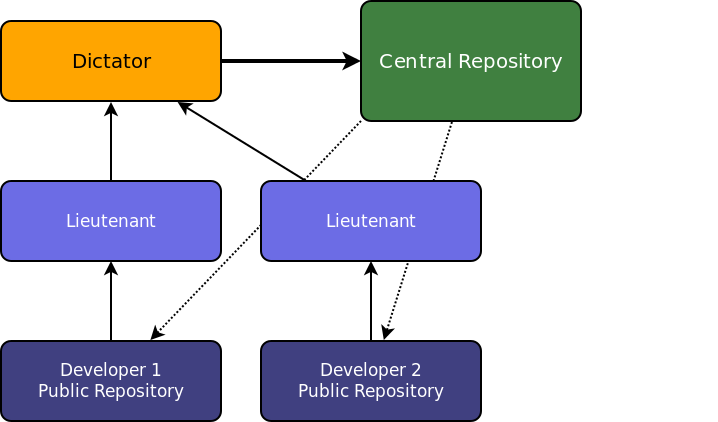
\includegraphics[width=0.5\textwidth]{img/Mod_Dictator}
  \caption{Dictator and Lieutenants Model}
  \label{fig:mod_dictator} 
\end{figure}

This workflow is an enhancement of the “Integration-Manager Workflow”. Instead of heaving a handful 
integration managers which are all responsible of the whole code base, you have a hierarchy of integration 
managers which are responsible for a certain module or subsystem. The topmost integration manager is called 
the “dictator”, and the integration managers on the levels below are called “lieutenants”.

The advantage of this model is that the dictator or a lieutenant does not have to check every change from 
each developer, instead he can just trust the lieutenants below him and pull changes from them. This model 
is not very common because it is very hierarchical and only starts to become effective if a project gets really big and complex.

An example is the Linux kernel, where Linus Torvalds acts as the dictator and the lieutenants are 
responsible for the different subsystems of the kernel.
